\subsection{Diseño del Sistema de Succión con Ventosa}

El sistema de efector final del kit incorpora un mecanismo de succión por vacío como alternativa al gripper mecánico original del PhantomX Pincher. Este sistema permite la manipulación de objetos ligeros mediante adhesión neumática, ampliando las capacidades didácticas del kit.

\subsubsection{Condiciones de Diseño}

Las restricciones y requerimientos técnicos del sistema de succión son:

\begin{itemize}
    \item Voltaje de alimentación disponible: 12 V DC (fuente del robot)
    \item Área típica de objetos a manipular: 25 mm × 25 mm
    \item Diámetro de ventosa seleccionada: 15 mm
    \item Restricción espacial: La bomba debe caber dentro de la base del manipulador
    \item Compatibilidad neumática: Conexión a mangueras de 6 mm de diámetro
\end{itemize}

\subsubsection{Evaluación de Bombas de Vacío}

Se evaluaron dos bombas de vacío miniatura compatibles con la alimentación de 12 V del robot:

\paragraph{Bomba Mini Air Pump 370A}

Microbomba de vacío diseñada específicamente para succión de aire. Utiliza motor tipo 370 con diafragma, genera vacío máximo de -65 kPa. Dimensiones compactas: aproximadamente 27 mm de diámetro × 58 mm de largo, peso 60 g. La boca de salida permite conexión directa a mangueras neumáticas de 6 mm sin acoples adicionales.

\paragraph{Bomba R385 Diaphragm Pump}

Bomba de diafragma diseñada para bombeo de agua, adaptable para aire. Opera entre 6 y 12 V DC con consumo de 0.5-1 A. Capacidad de succión máxima: 2 m de columna de agua (equivalente a aproximadamente 19.6 kPa). Dimensiones: 90 mm × 40 mm × 35 mm, peso 112 g. Diámetro de boca: 7-8.5 mm externo, requiere acople para mangueras de 6 mm.

\subsubsection{Comparación Técnica}

La Tabla \ref{tab:comparacion_bombas} resume las especificaciones técnicas de ambas bombas.

\begin{table}[H]
\centering
\caption{Comparación de especificaciones técnicas de bombas de vacío}
\label{tab:comparacion_bombas}
\small
\begin{tabular}{|l|c|c|}
\hline
\textbf{Parámetro} & \textbf{Bomba 370A} & \textbf{Bomba R385} \\
\hline
Voltaje nominal & DC 12 V & DC 6-12 V \\
Corriente & 280-420 mA & 500-700 mA \\
Potencia aproximada & 3.4-5 W & 4.8-6 W \\
Tipo de bomba & Vacío (aire) & Diafragma (agua/aire) \\
Vacío máximo & -65 kPa & -19.6 kPa (2 m col. agua) \\
Flujo de aire & 3.5-4.5 LPM & 1.5-2 L/min \\
Dimensiones & Ø27 × 58 mm & 90 × 40 × 35 mm \\
Peso & 60 g & 112 g \\
Ruido & 55-60 dB & $<$30 dB (agua) \\
Diámetro de boca & 4.2-6 mm & Int. 6 mm, ext. 8.5 mm \\
Conexión neumática & Directa Ø6 mm & Requiere acople \\
Vida útil & $>$50,000 ciclos & 2,500 h \\
\hline
\end{tabular}
\end{table}

\subsubsection{Análisis de Capacidad de Levantamiento}

Para determinar la capacidad de cada bomba, se calculó la fuerza de succión generada sobre el área efectiva de la ventosa.

\paragraph{Datos del Sistema}

\begin{itemize}
    \item Diámetro de ventosa: $d = 15$ mm $= 0.015$ m
    \item Radio de ventosa: $r = 7.5$ mm $= 0.0075$ m
    \item Área efectiva: $A = \pi r^{2} = \pi \times (0.0075)^{2} = 1.7671 \times 10^{-4}$ m$^{2}$
    \item Aceleración gravitacional: $g = 9.81$ m/s$^{2}$
\end{itemize}

\paragraph{Modelo Teórico}

La fuerza de succión se calcula mediante:

\begin{equation}
F = \Delta P \times A
\end{equation}

donde $F$ es la fuerza de succión [N], $\Delta P$ es la presión de vacío generada [Pa], y $A$ es el área efectiva de la ventosa [m$^{2}$].

La masa máxima levantable se obtiene de:

\begin{equation}
m = \frac{F}{g}
\end{equation}

\paragraph{Cálculo para Bomba 370A}

Vacío máximo: -65 kPa = 65,000 Pa

\begin{align}
F_{370} &= 65{,}000 \times 1.7671 \times 10^{-4} = 11.49 \text{ N} \\
m_{370} &= \frac{11.49}{9.81} = 1.17 \text{ kg}
\end{align}

\paragraph{Cálculo para Bomba R385}

Capacidad de succión: 2 m de columna de agua

Conversión a presión:
\begin{equation}
\Delta P = \rho \cdot g \cdot h = 1{,}000 \times 9.81 \times 2 = 19{,}620 \text{ Pa} \approx 19.6 \text{ kPa}
\end{equation}

\begin{align}
F_{R385} &= 19{,}620 \times 1.7671 \times 10^{-4} = 3.47 \text{ N} \\
m_{R385} &= \frac{3.47}{9.81} = 0.354 \text{ kg} = 354 \text{ g}
\end{align}

\paragraph{Resumen de Resultados}

La Tabla \ref{tab:capacidad_levantamiento} resume la capacidad de levantamiento de ambas bombas.

\begin{table}[H]
\centering
\caption{Capacidad de levantamiento de bombas de vacío}
\label{tab:capacidad_levantamiento}
\small
\begin{tabular}{|l|c|c|}
\hline
\textbf{Parámetro} & \textbf{Bomba 370A} & \textbf{Bomba R385} \\
\hline
Vacío máximo (kPa) & -65 & -19.6 \\
Fuerza de succión (N) & 11.49 & 3.47 \\
Masa máxima teórica (kg) & 1.17 & 0.354 \\
Factor de seguridad ×0.5 & 0.585 kg & 0.177 kg \\
\hline
\end{tabular}
\end{table}

\paragraph{Consideraciones Prácticas}

Los valores calculados son teóricos y asumen sellado perfecto entre ventosa y objeto. En la práctica, la fuerza efectiva se reduce por:

\begin{itemize}
    \item Fugas de aire entre ventosa y superficie
    \item Rugosidad superficial del objeto
    \item Pérdidas en mangueras y conexiones neumáticas
    \item Deformación de la ventosa
    \item Tiempo de establecimiento del vacío
\end{itemize}

Se recomienda aplicar un factor de seguridad de 2 (utilizar 50\% de capacidad teórica). Con este factor, la bomba 370A puede levantar de manera confiable objetos de hasta 585 g, mientras que la R385 está limitada a aproximadamente 177 g.

\subsubsection{Justificación de la Selección}

La bomba 370A fue seleccionada por las siguientes razones:

\begin{enumerate}
    \item \textbf{Capacidad de vacío superior}: Genera -65 kPa, más de tres veces mayor que los -19.6 kPa de la R385, resultando en fuerza de succión de 11.49 N frente a 3.47 N
    
    \item \textbf{Diseño compacto}: Dimensiones de Ø27 × 58 mm y peso de 60 g, significativamente más pequeña que la R385 (90 × 40 × 35 mm, 112 g), facilitando integración en la base del robot
    
    \item \textbf{Conexión directa}: Boca compatible con mangueras de 6 mm sin acoples adicionales. La R385 requiere acople intermedio
    
    \item \textbf{Menor consumo energético}: Consume 280-420 mA frente a 500-1,000 mA de la R385, reduciendo carga sobre la fuente de alimentación
    
    \item \textbf{Diseño específico para vacío}: Optimizada para succión de aire, a diferencia de la R385 diseñada para bombeo de agua
    
    \item \textbf{Costo}: Precio más accesible, compatible con el presupuesto del proyecto
\end{enumerate}

\subsubsection{Selección de Ventosa}

La selección de la ventosa se fundamentó en dos criterios principales: disponibilidad comercial en el mercado nacional e internacional, y compatibilidad dimensional con los objetos a manipular.

\paragraph{Criterios de Dimensionamiento}

Los objetos de clasificación contemplados para el kit poseen dimensiones estándar de 25 mm × 25 mm. Para garantizar un margen de seguridad adecuado que permita variaciones en el posicionamiento del manipulador y tolerancias en la ubicación de los objetos, se estableció que la ventosa debía proporcionar una holgura mínima de 5 mm respecto a los bordes del objeto.

Con base en este criterio, se seleccionó una ventosa de 15 mm de diámetro, que proporciona:

\begin{itemize}
    \item Holgura lateral: $\frac{25 - 15}{2} = 5$ mm por cada lado
    \item Área de contacto suficiente para garantizar adhesión confiable
    \item Compatibilidad con objetos de dimensiones variables entre 15 mm y 30 mm aproximadamente
\end{itemize}

Esta configuración permite que, incluso con desalineamientos moderados del manipulador (±5 mm), la ventosa pueda establecer contacto efectivo con la superficie del objeto y generar el vacío necesario para su levantamiento.

\paragraph{Ventosa Seleccionada}

Se seleccionó la ventosa modelo PAK-15, disponible comercialmente a través de proveedores internacionales. Esta ventosa presenta las siguientes características:

\begin{itemize}
    \item Diámetro: 15 mm
    \item Material: Silicona o caucho nitrílico (NBR), resistente a deformación y degradación
    \item Conexión: Compatible con mangueras neumáticas de 4-6 mm de diámetro interno
    \item Tipo: Ventosa plana de propósito general, adecuada para superficies lisas o ligeramente texturizadas
    \item Costo: Accesible, compatible con el presupuesto del proyecto
\end{itemize}

La ventosa PAK-15 es ampliamente utilizada en sistemas de automatización ligera y pick-and-place debido a su versatilidad, durabilidad y facilidad de instalación. Su diseño permite un sellado efectivo sobre superficies planas, maximizando la transmisión del vacío generado por la bomba 370A hacia el objeto a manipular.

\paragraph{Consideraciones de Integración}

La ventosa se conecta a la bomba de vacío mediante una manguera neumática de 6 mm de diámetro exterior (4 mm de diámetro interior). Esta configuración minimiza las pérdidas de vacío y garantiza tiempos de respuesta rápidos durante las operaciones de succión y liberación de objetos.

El montaje de la ventosa en el efector final del manipulador se realiza mediante un soporte diseñado específicamente que permite:

\begin{itemize}
    \item Alineación precisa con el eje vertical del manipulador
    \item Conexión segura de la manguera neumática sin restricciones de movimiento
    \item Acceso visual de la cámara superior a los objetos durante la aproximación
    \item Reemplazo rápido de la ventosa en caso de desgaste o daño
\end{itemize}

\subsubsection{Sistema Completo de Succión por Vacío}

El sistema de succión por vacío integra múltiples subconjuntos y componentes neumáticos que trabajan coordinadamente para permitir la manipulación de objetos mediante adhesión. La Figura \ref{fig:ensambleSuccion} presenta una vista general del sistema completo instalado en el kit.

\begin{figure}[H]
    \centering
    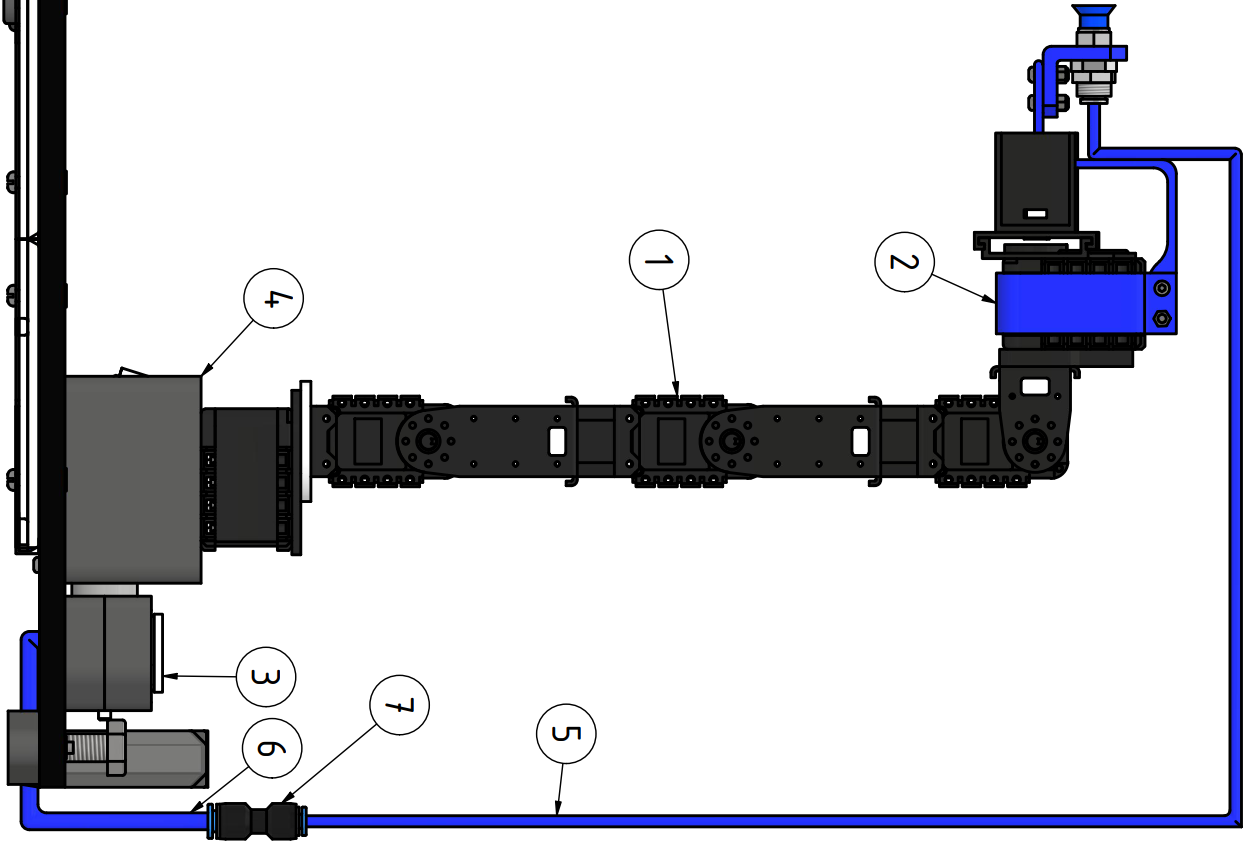
\includegraphics[width=0.95\textwidth]{06disenoConceptual/img/succion/ensambleSuccion.png}
    \caption{Sistema completo de succión por vacío integrado en el kit. (1) Brazo robótico PhantomX Pincher AX-12, (2) Subconjunto de gripper de succión montado en el efector final, (3) Subconjunto de base de bomba de vacío, (4) Subconjunto de base del manipulador, (5) Manguera neumática M4 × 1 m conectando bomba y gripper, (6) Manguera neumática M6 × 30 cm (conexión auxiliar), (7) Acople reductor de 6 mm a 4 mm para compatibilidad entre mangueras y ventosa.}
    \label{fig:ensambleSuccion}
\end{figure}

\begin{table}[H]
\centering
\caption{Componentes principales del sistema de succión}
\label{tab:sistema_succion}
\small
\begin{tabular}{|c|l|c|}
\hline
\textbf{\#} & \textbf{Componente} & \textbf{Cant.} \\
\hline
1 & Brazo robótico PhantomX Pincher AX-12 & 1 \\
2 & Subconjunto de gripper de succión & 1 \\
3 & Subconjunto de base de bomba de vacío & 1 \\
4 & Subconjunto de base de manipulador & 1 \\
5 & Manguera neumática M4 × 1 m & 1 \\
6 & Manguera neumática M6 × 30 cm & 1 \\
7 & Acople reductor 6 mm a 4 mm & 1 \\
\hline
\end{tabular}
\end{table}

El sistema está compuesto principalmente por el subconjunto del gripper de succión (que incluye la ventosa y su soporte), el subconjunto de la bomba de vacío (que aloja la bomba 370A), las mangueras neumáticas que conectan ambos elementos, y el acople reductor que garantiza compatibilidad entre diferentes diámetros. Los demás elementos listados (base del manipulador y brazo robótico) se incluyen en la descripción por su función de soporte estructural y anclaje de los componentes neumáticos.

\subsubsection{Diseño del Subconjunto de Gripper de Succión}

El subconjunto del gripper de succión constituye el efector final del sistema de vacío. Su diseño permite la coexistencia del gripper mecánico original con el sistema de succión, facilitando el cambio rápido entre ambos modos de operación sin necesidad de desmontar completamente ninguno de los dos sistemas.

\begin{figure}[H]
    \centering
    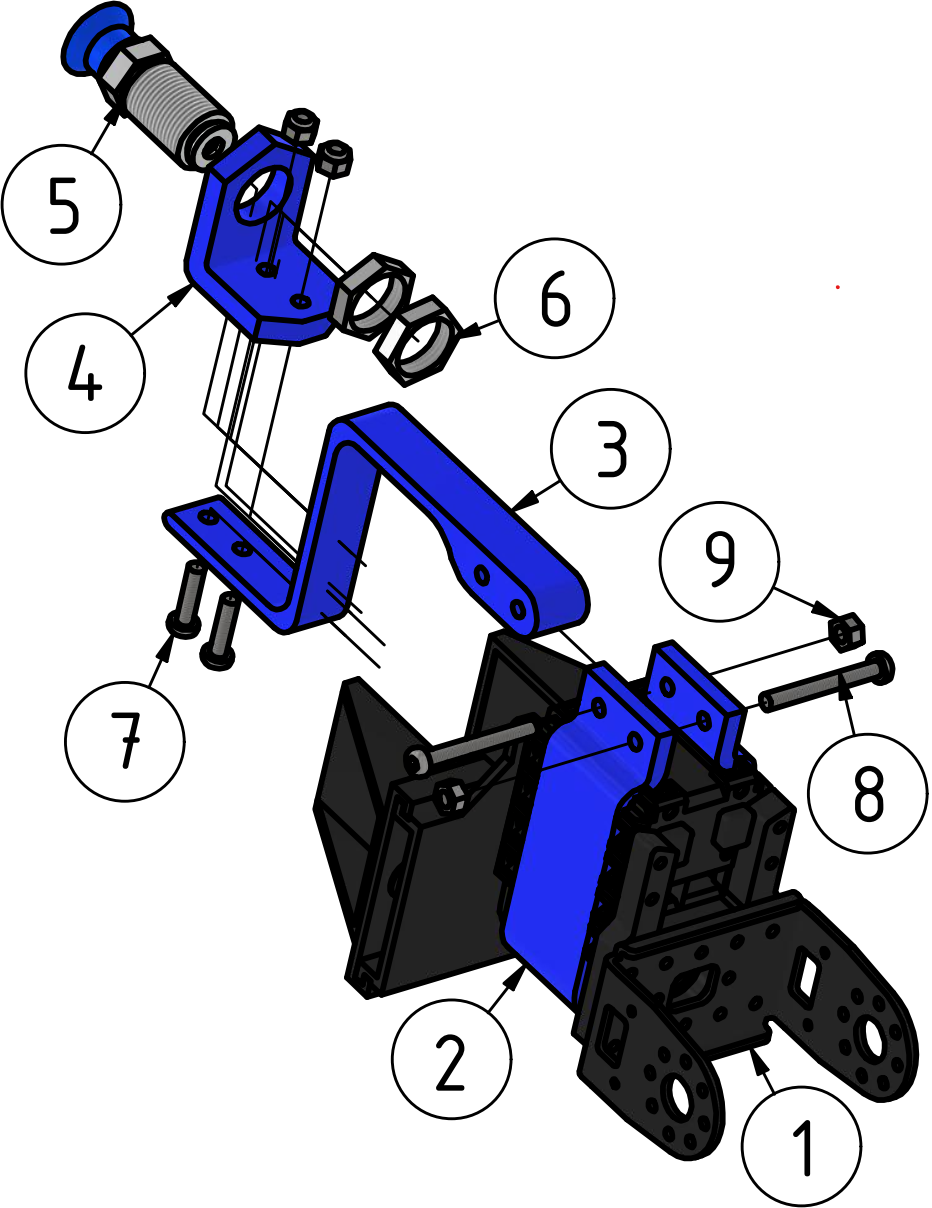
\includegraphics[width=0.65\textwidth]{06disenoConceptual/img/succion/ensambleVentosa.png}
    \caption{Ensamble explosionado del subconjunto de gripper de succión. (1) Gripper de pinza original del robot, (2) Pieza de anclaje al motor del gripper fabricada mediante FDM, (3) Pieza de extensión de ventosa que proporciona separación vertical, (4) Pieza de anclaje de ventosa con conexión neumática, (5) Ventosa PAK-15 de 15 mm de diámetro, (6) Tuercas M12 × 4 mm con paso de rosca 1 mm, (7) Tornillos M3 × 12 mm, (8) Tornillos M3 × 25 mm, (9) Tuercas de seguridad M3 (4 unidades).}
    \label{fig:ensambleVentosa}
\end{figure}

\begin{table}[H]
\centering
\caption{Lista de materiales del subconjunto de gripper de succión}
\label{tab:bom_gripper_succion}
\small
\begin{tabular}{|c|l|c|l|l|}
\hline
\textbf{\#} & \textbf{Componente} & \textbf{Cant.} & \textbf{Fabricación} & \textbf{Material} \\
\hline
1 & Gripper de pinza & 1 & --- & --- \\
2 & Pieza de anclaje a gripper & 1 & FDM & PLA/ABS \\
3 & Pieza de extensión de ventosa & 1 & FDM & PLA/ABS \\
4 & Pieza de anclaje de ventosa & 1 & FDM & PLA/ABS \\
5 & Ventosa PAK-15 & 1 & Comercial & Silicona/NBR \\
6 & Tuerca M12 × 4 mm (paso 1 mm) & 2 & Comercial & Acero \\
7 & Tornillo M3 × 12 mm & 2 & Comercial & Acero \\
8 & Tornillo M3 × 25 mm & 2 & Comercial & Acero \\
9 & Tuerca M3 de seguridad & 4 & Comercial & Acero \\
\hline
\end{tabular}
\end{table}

\paragraph{Estrategia de Diseño Modular}

El diseño del gripper de succión se fundamentó en el principio de modularidad, permitiendo la conversión rápida entre modo de pinza mecánica y modo de succión sin requerir desmontaje extensivo. La pieza de anclaje al gripper se fabrica mediante FDM y se monta directamente sobre el servomotor del gripper original, permaneciendo fija mediante ajuste por fricción sin necesidad de tornillería adicional.

El resto del sistema de succión (extensión, anclaje de ventosa y ventosa) se atornilla a esta pieza base mediante dos tornillos M3. Esta configuración permite:

\begin{itemize}
    \item Cambio entre pinza mecánica y ventosa mediante remoción/instalación de solo dos tornillos
    \item Preservación del gripper original sin modificaciones permanentes
    \item Tiempo de cambio de configuración inferior a 2 minutos
    \item Posibilidad de almacenar el sistema no utilizado sin ocupar espacio significativo
\end{itemize}

\paragraph{Función de la Pieza de Extensión}

La pieza de extensión cumple una función crítica al proporcionar separación vertical entre la ventosa y los dedos del gripper mecánico. Esta separación garantiza:

\begin{itemize}
    \item Campo visual libre para la cámara superior durante aproximación al objeto
    \item Prevención de colisiones entre ventosa y objetos durante operaciones de depósito
    \item Espacio suficiente para alojamiento de la manguera neumática
    \item Alineación vertical precisa de la ventosa con el eje del manipulador
\end{itemize}

\paragraph{Centrado de la Ventosa}

El diseño garantiza que la ventosa quede centrada respecto al eje longitudinal del gripper, como se observa en las vistas ortogonales de la Figura \ref{fig:vistasVentosa}. Este centrado es fundamental para:

\begin{itemize}
    \item Simplificar la programación de trayectorias (no requiere compensación de offset)
    \item Maximizar la repetibilidad del posicionamiento
    \item Facilitar la calibración visual del sistema
    \item Distribuir uniformemente las cargas durante el levantamiento
\end{itemize}

\begin{figure}[H]
    \centering
    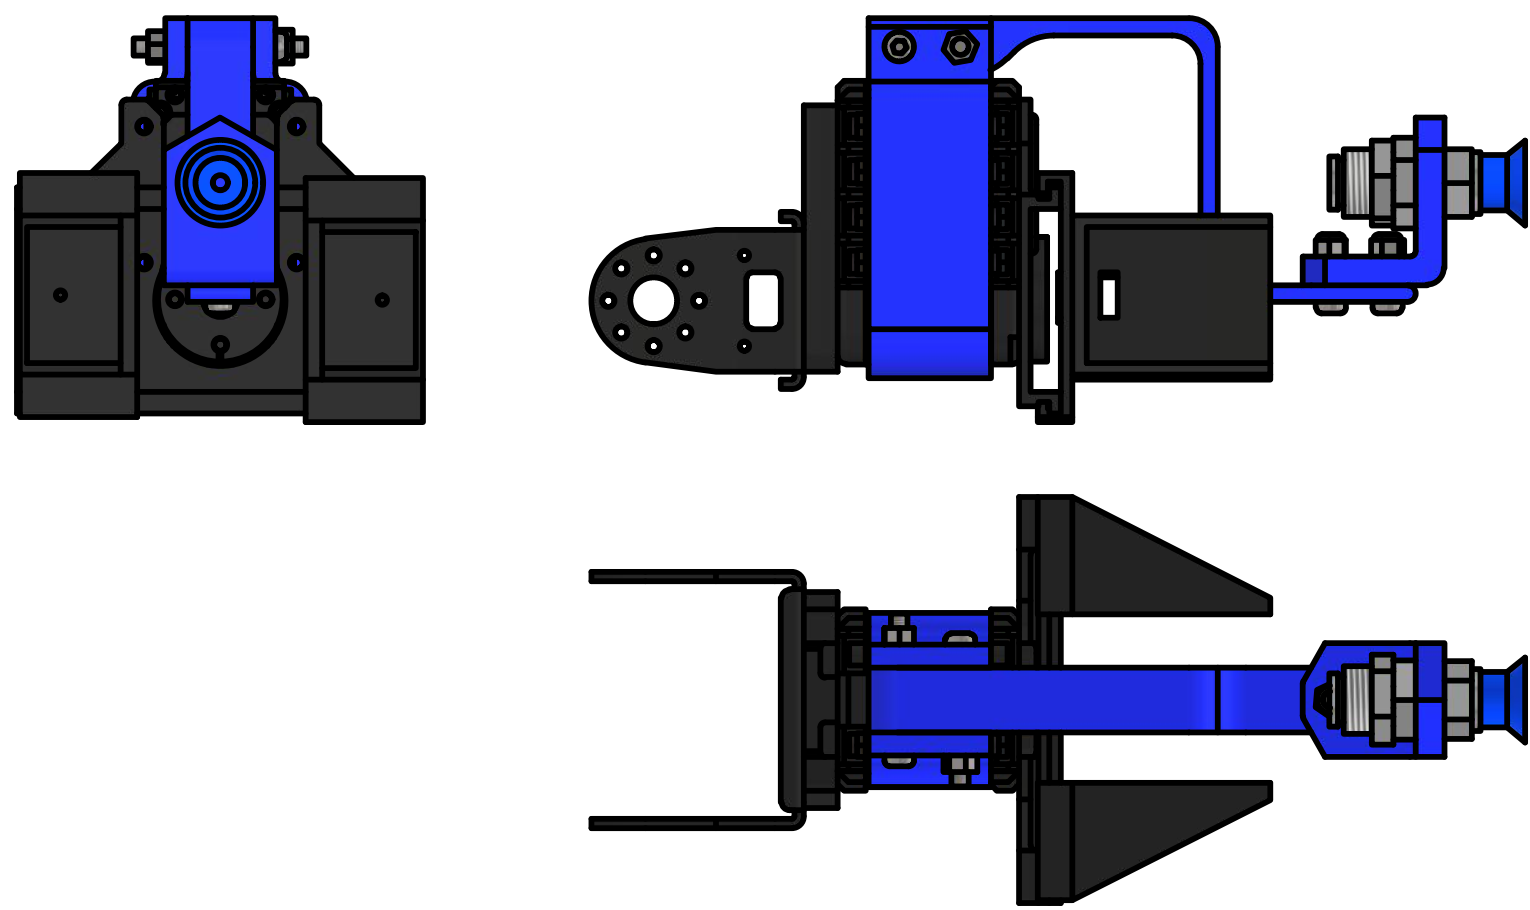
\includegraphics[width=0.9\textwidth]{06disenoConceptual/img/succion/vistasVentosa.png}
    \caption{Vistas ortogonales del gripper de succión. Vista frontal (izquierda): se observa el centrado de la ventosa respecto al eje del gripper. Vista lateral (superior derecha): se aprecia la extensión vertical y la conexión neumática. Vista inferior (inferior derecha): se muestra la disposición de la ventosa y el ruteo de la manguera hacia la conexión lateral.}
    \label{fig:vistasVentosa}
\end{figure}

\subsubsection{Diseño del Subconjunto de Base de Bomba de Vacío}

El subconjunto de la base de bomba de vacío cumple funciones duales: por un lado, proporciona el montaje estructural de la bomba 370A a la plataforma base; por otro, integra el sistema de identificación numérica del kit.

\begin{figure}[H]
    \centering
    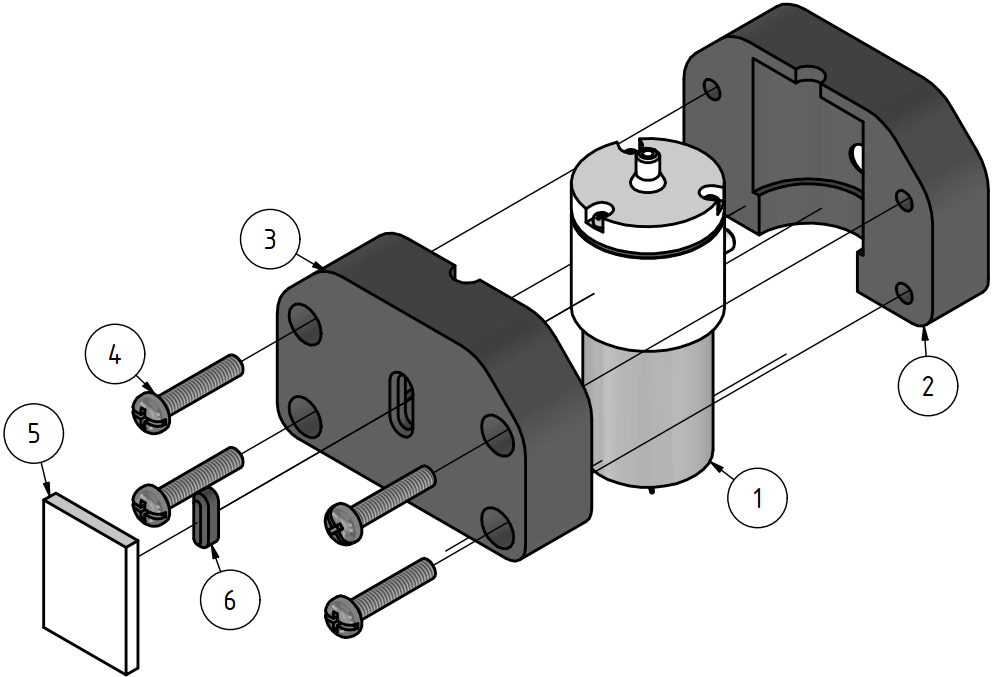
\includegraphics[width=0.6\textwidth]{06disenoConceptual/img/succion/ensambleBombaVacio.png}
    \caption{Ensamble explosionado del subconjunto de base de bomba de vacío. (1) Bomba de vacío 370A, (2) Parte inferior de la base fabricada mediante FDM que se atornilla a la plataforma, (3) Parte superior de la base que abraza la bomba cilíndrica, (4) Tornillos M4 × 25 mm para fijación a insertos roscados de la plataforma, (5) Placa identificadora numérica del kit, (6) Clip de encaje para retención de la placa.}
    \label{fig:ensambleBombaVacio}
\end{figure}

\begin{table}[H]
\centering
\caption{Lista de materiales del subconjunto de base de bomba de vacío}
\label{tab:bom_base_bomba}
\small
\begin{tabular}{|c|l|c|l|l|}
\hline
\textbf{\#} & \textbf{Componente} & \textbf{Cant.} & \textbf{Fabricación} & \textbf{Material} \\
\hline
1 & Bomba de vacío 370A & 1 & Comercial & --- \\
2 & Parte inferior de base & 1 & FDM & ABS/PLA \\
3 & Parte superior de base & 1 & FDM & ABS/PLA \\
4 & Tornillo M4 × 25 mm & 4 & Comercial & Acero \\
5 & Placa identificadora & 1 & FDM & PLA/ABS \\
6 & Clip de encaje & 1 & FDM & PLA/ABS \\
\hline
\end{tabular}
\end{table}

\paragraph{Configuración de Montaje}

La base se diseñó en dos piezas que abrazan el cuerpo cilíndrico de la bomba 370A:

\begin{itemize}
    \item \textbf{Parte inferior}: Se atornilla directamente a la plataforma base mediante cuatro tornillos M4 × 25 mm que se enroscan en insertos roscados. Incorpora una semicavidad que aloja la mitad inferior de la bomba
    \item \textbf{Parte superior}: Completa el abrazo de la bomba y se fija a la parte inferior mediante el mismo sistema de tornillería que atraviesa la plataforma
\end{itemize}

Esta configuración permite la instalación y remoción de la bomba sin necesidad de desmontar completamente la base, facilitando operaciones de mantenimiento o reemplazo.

\paragraph{Sistema de Identificación}

La placa identificadora se monta en la superficie superior de la base de la bomba mediante un clip de encaje plástico. Para garantizar retención permanente, se aplica adhesivo de cianoacrilato (tipo Superbonder) en la interfaz entre placa y clip. Esta ubicación fue seleccionada por:

\begin{itemize}
    \item Visibilidad desde múltiples ángulos de aproximación al kit
    \item Protección contra contacto accidental durante operaciones normales
    \item Facilidad de lectura sin interferencia con componentes móviles
    \item Posibilidad de reemplazo en caso de daño
\end{itemize}

El sistema de identificación permite distinguir inequívocamente cada uno de los siete kits, facilitando la gestión de inventario, asignación en actividades de laboratorio, y trazabilidad de mantenimiento.

El diseño completo del sistema de succión por vacío representa una solución integrada que equilibra funcionalidad, modularidad, facilidad de manufactura y compatibilidad con el sistema mecánico original del PhantomX Pincher, proporcionando al kit capacidades ampliadas de manipulación mediante un efector final intercambiable.